\section{Differential Datalog (DDlog)}\label{sec-ddlog}

\subsection{Differential computation}

\begin{figure}[t]
  \begin{minipage}{.5\textwidth}
    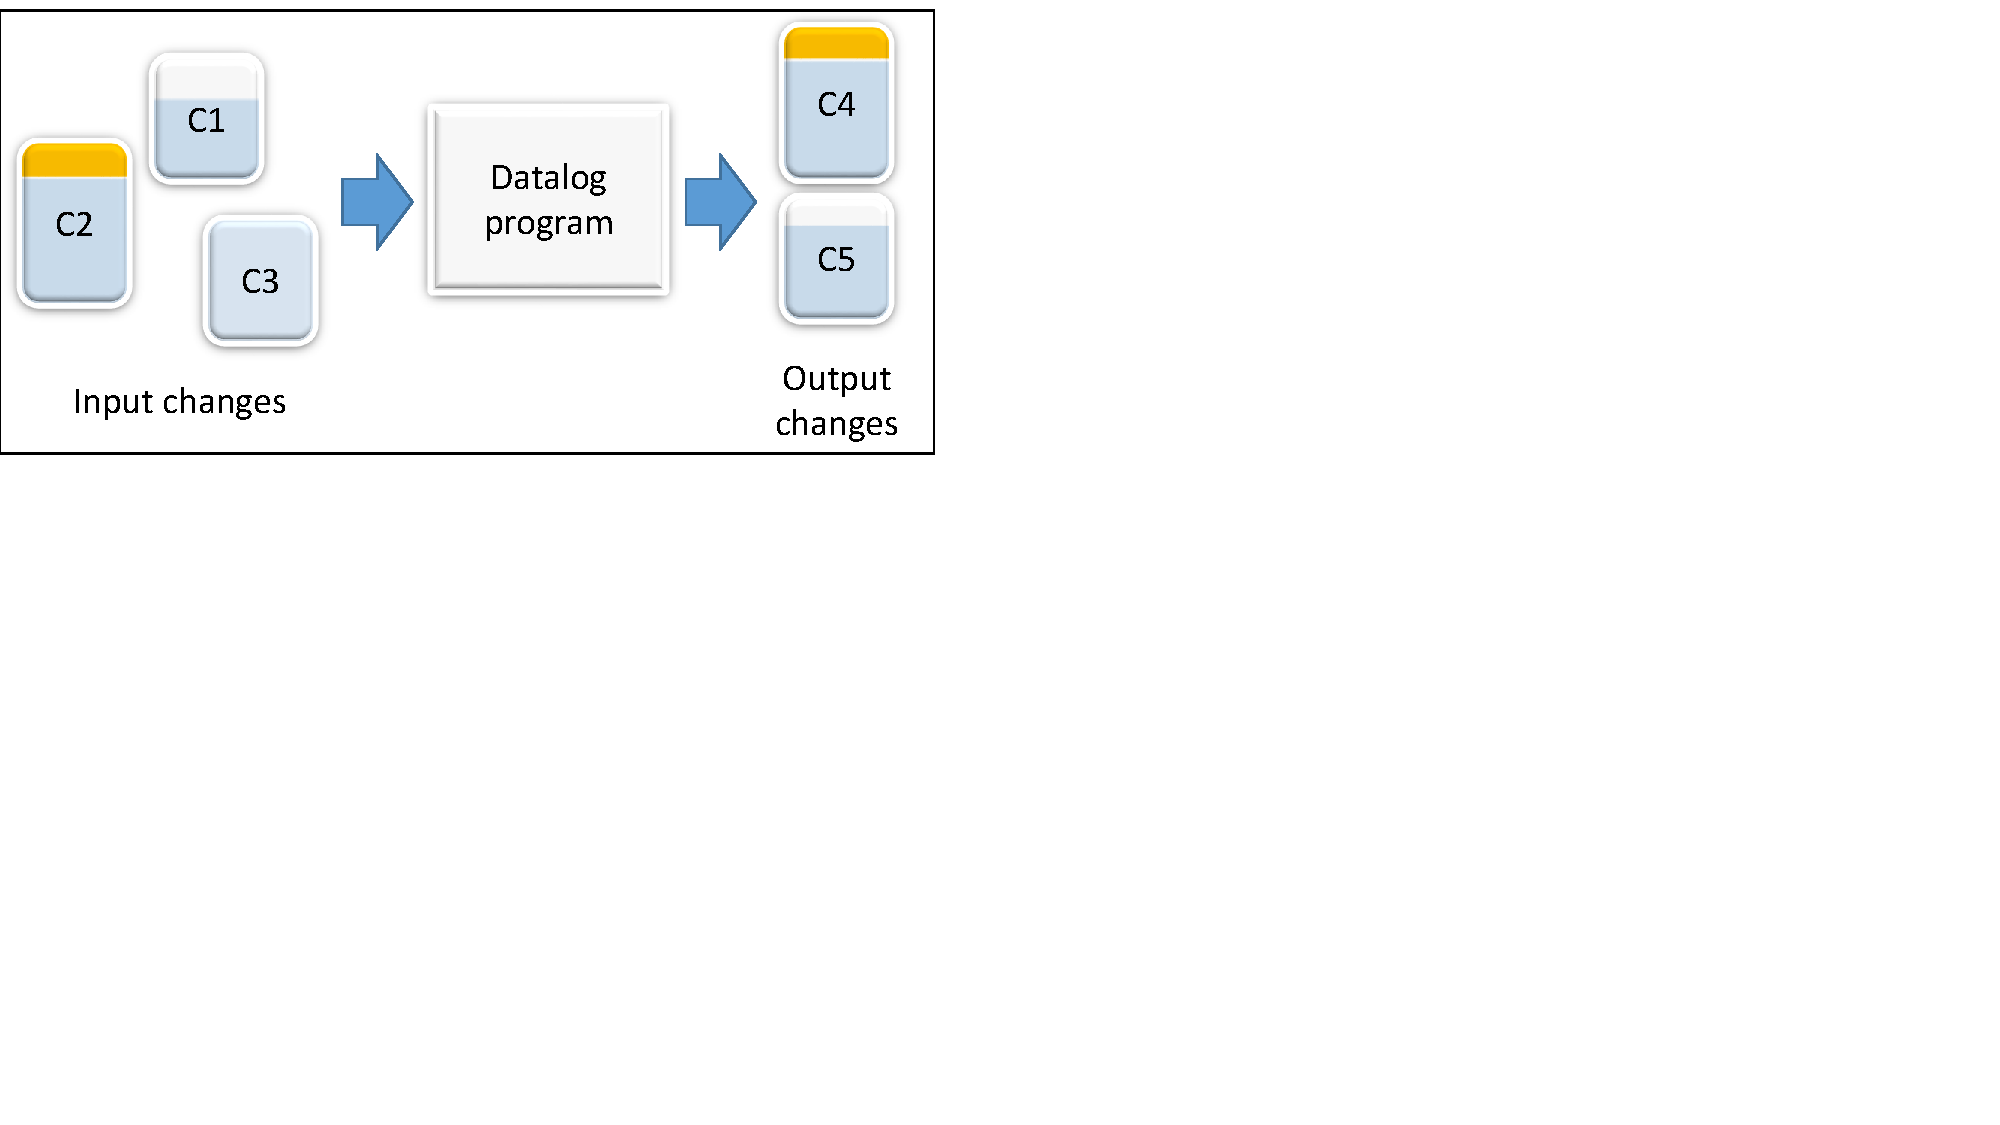
\includegraphics[width=\columnwidth,clip=true,trim=0in 1.7in 6.5in
      0in]{differential.pdf}
    \caption{Differential computation.\label{fig:differential}}
  \end{minipage} \hfill
  \begin{minipage}{.5\textwidth}
    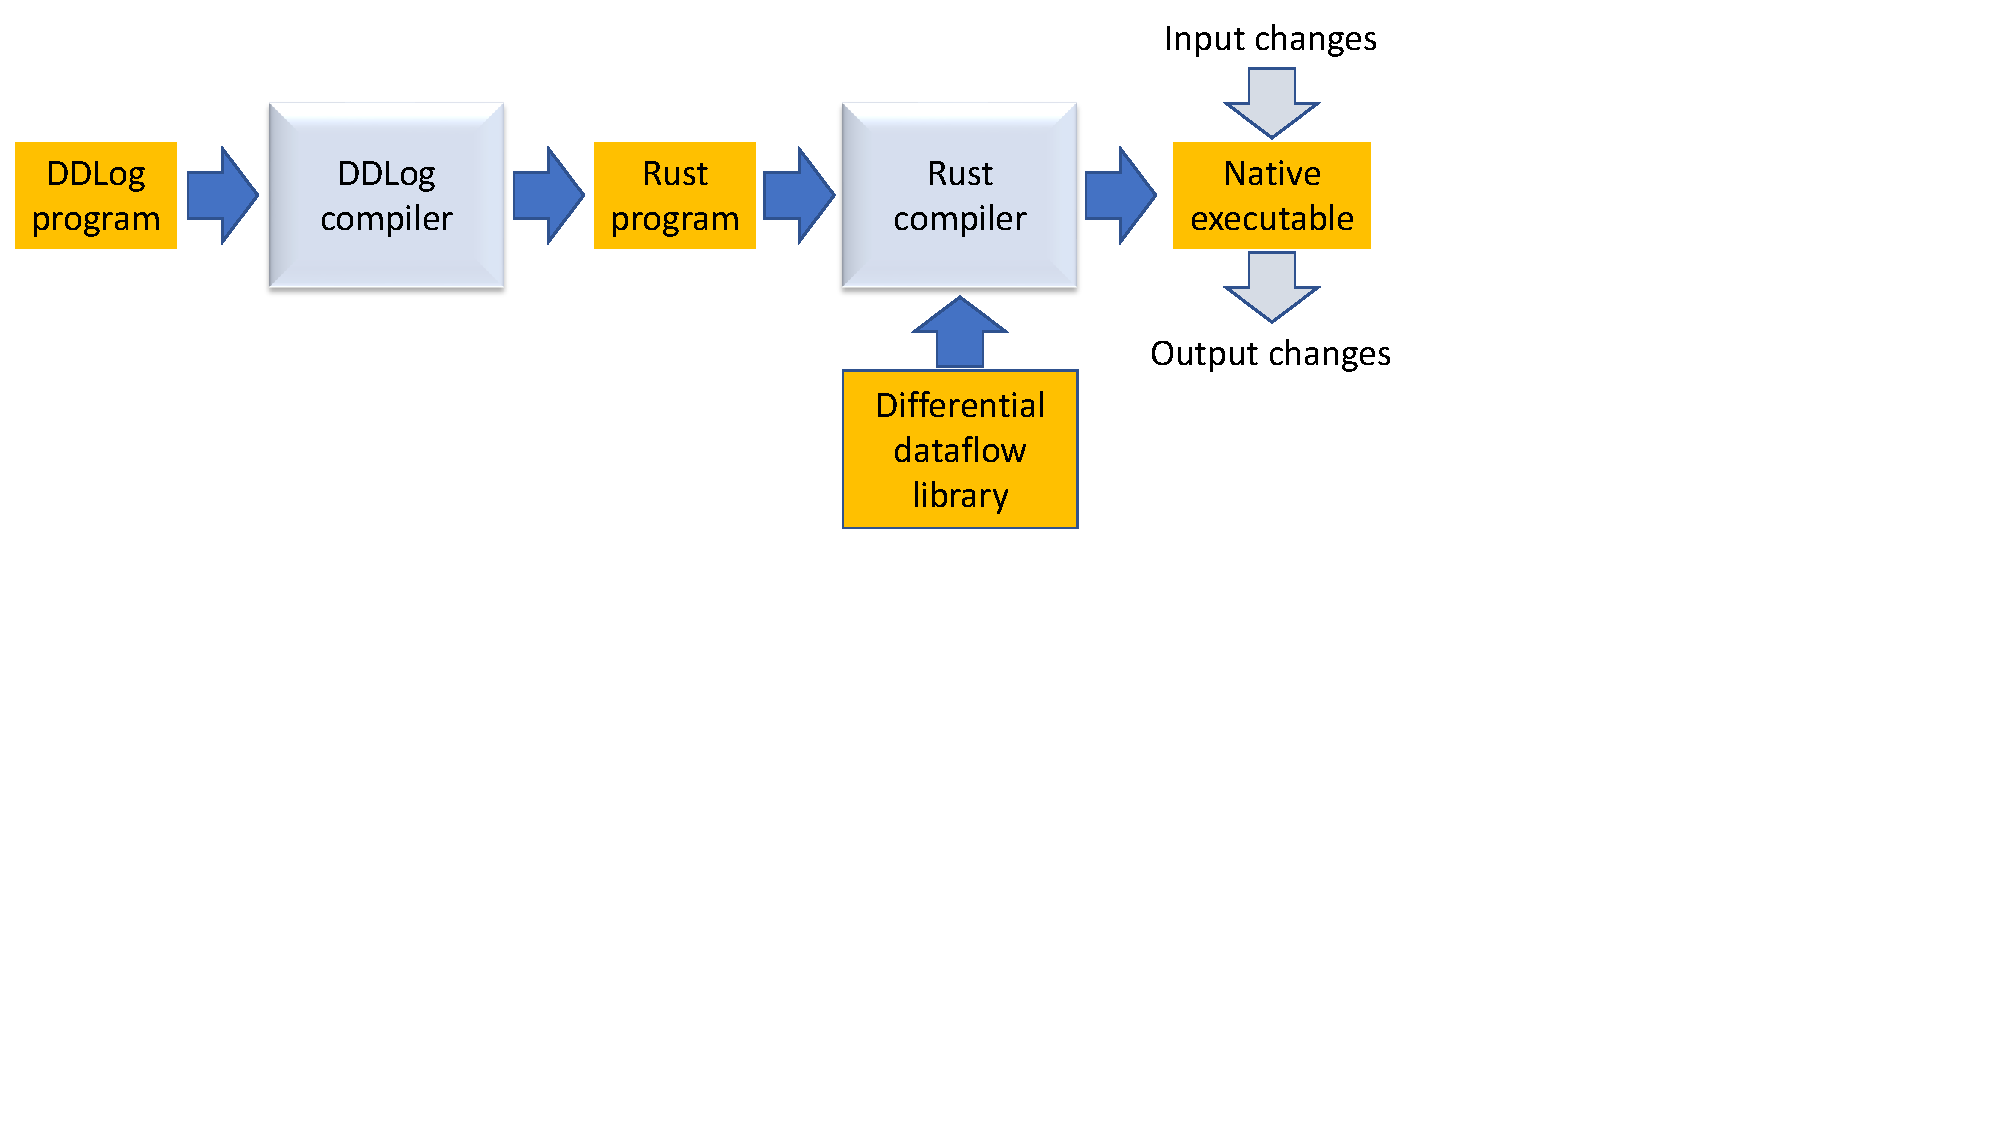
\includegraphics[width=\columnwidth,clip=true,trim=0in 4in 4in
      0in]{compiler-flow.pdf}
    \caption{Using DDlog.\label{fig:compiler-flow}}
  \end{minipage}
\end{figure}

A DDlog program operates on typed relations.  The programmer defines a
set of rules to compute a set of output relations based on input
relations (Figure~\ref{fig:differential}).  Rules are evaluated
incrementally: given a set of \emph{changes} to the input relations
(insertions or deletions), DDlog produces a set of changes to the
output relations (expressed also as insertions or deletions).

In this section we give a brief overview of the language; we refer the
reader to the DDlog language reference~\cite{ddlog-manual} for a
detailed presentation of the syntax, and to the DDlog
tutorial~\cite{ddlog-tutorial}.

\subsection{Syntax}

DDlog is case-sensitive.  Relation, constructor, and type variable
names must start with upper-case ASCII letters; variable, function,
and argument names must start with lower-case ASCII letters or
underscore.  A type variable name must be prefixed with a tick
(\texttt{'}). A type name can start with either an upper-case or a
lower-case letter or underscore.  Names must be unique within a scope.

\subsection{Language restrictions}

DDlog support recursion with stratified negation.  This is natural
restriction, also present in the SQL standard.

\subsection{Type system}

DDlog is a strongly-typed language.  DDlog performs type inference,
but users can specify the types of expressions explicitly as well.
All programs are type-checked statically.  The type system is inspired
by Haskell, and supports a rich set of types.  Base types include
Booleans, bit-strings, e.g., \texttt{bit<32>}, infinite-precision
integers \texttt{bigint}, UTF-8 strings.  Derived types are tuples,
structures, and tagged unions (which generalize enumerated types).  We
do not support recursive types (like lists or trees).

Figure~\ref{fig:types} shows several type declarations.  DDlog
supports also generic types; type variables are preceded by a tick:
\texttt{'A}.  The language contains a built-in reference type
\texttt{Ref<'T>}.  Unlike other languages, two references are equal if
the objects referred are equal; thus references do not alter the
nature of Datalog in any significant way.  References can be used to
reduce memory consumption when complex objects are stored in multiple
relations.

\begin{figure}[t]
  \small
\begin{lstlisting}[language=ddlog]
// A tagged-union type
typedef IPAddress = IPv4Address{ipv4addr: bit<32>} // 32-bit vector
                  | IPv6Address{ipv6addr: bit<128>}
// A generic option type
typedef Option<'A> = None
                   | Some{value: 'A}
typedef OptionalIPAddress = Option<IPAddress>                   
\end{lstlisting}
\caption{Some type declarations in DDlog.\label{fig:types}}
\end{figure}

\subsection{Relations}

Relations are strongly typed; the value in each column must have a
statically-determined type.  There are three kinds of relations in
DDlog:
\begin{description}
\item[Input relations:] the contents of these relations is provided by
  the environment of the program.
\item[Output relations:] these must be computed by the DDlog program, and the
  DDlog runtime will inform the environment of any changes that
  occur in these relations.
\item[Intermediate results:] these must be also computed by the DDlog
  program, but the environment cannot query the contents of these
  relations.
\end{description}

Figure~\ref{fig:relations} shows several relation declarations.  An
input relation may declare an optional primary key --- which is a set
of columns that can be used to delete entries more efficiently,
specifying only the key.

\begin{figure}[t]
  \small
  \begin{lstlisting}[language=ddlog]
relation R(f1: string, f2: bigint) primary key (r) r.f1

// Another way to declare the same relation starting
// from an existing type
typedef R = R{f1: string, f2: bigint}
relation R[R] primary key (r) r.f1

// Relation StrRX contains string representations of
// all tuples in R that have the first field "x".
// Uses filtering, conjunction, inline variables and expression.
relation StrRX(s: string) :- r in R(.f1 = "x"),
                             var s = r.f1 ++ r.f2.
  \end{lstlisting}
  \caption{Example relation declarations.\label{fig:relations}}
\end{figure}

\subsection{Expression language}

DDlog is an expression-oriented language; programs are composed of
expressions, that evaluate to ground values.  Sequential composition
of two expressions (written using semicolon) evaluates to the last
expression.

The arithmetic types (\texttt{bigint} and \texttt{bit<N>}) provide a
rich set of arithmetic operations, including bit-selection
\texttt{v[15:8]}, shifting, and concatenation.

All primitive types contain built-in conversions to strings, and users
can implement string conversion functions for user-defined types
(like Java's toString() method).

Expressions enclosed within \texttt{\$\{...\}} in a string literal are
\emph{interpolated}: they are evaluated at run-time, converted to
strings and substituted; this is a feature inspired by JavaScript; for
example \texttt{"x+y=\$\{x+y\}"}.

\texttt{if} is an expression, similar to the C/Java \texttt{?:}
construct; in consequence the \texttt{else} branch is mandatory.
Inspired from ML and Haskell is the \texttt{match} expression which
simultaneously performs pattern-matching against type constructors or
values and value binding.  Figure~\ref{fig:function} shows how a
\texttt{match} expression uses a nested pattern to extract a byte from
an \texttt{OptionalIPAddress}.  This pattern binds the \texttt{addr}
variable.  In programmers can use \texttt{for} loops to iterate
over elements in collections.  

\subsection{(Pure) functions}

\begin{figure}[t]
  \small
  \begin{lstlisting}[language=ddlog]
function lastByte(a: OptionalIPAddress): bit<8> = {
  match (a) {
    None -> 0,
    Option{.Some = IPv4Address{.ipv4addr{addr}}} -> addr[7:0],
    Option{.Some = IPv6Address{.ipv6addr{addr}}} -> addr[7:0]
  }
}      
  \end{lstlisting}
  \caption{A simple pure function in DDlog.\label{fig:function}}
\end{figure}

Users can write functions using a simple imperative language embedded
directly into DDlog.  A function is shown in
Figure~\ref{fig:function}.  However, functions must be pure --- they
cannot have side-effects.  Recursive functions are not supported.
Users and libraries can declare prototypes of \texttt{extern}
functions, which can be implemented in Rust.  The compiler will also
assume that extern functions are pure.  Users can declare local
variables; local variables are typed and lexically scoped.

\subsection{Collections}

The DDlog standard library contains three built-in generic collection
types (implemented natively in Rust): \texttt{Vec<'T>},
\texttt{Set<'T>} and \texttt{Map<'T>}.  Values of these types can be
contained as first-class values within relations.  Equality for values
of these types is defined as expected, element-wise.  In theory such
types are not necessary, since collections within relations could be
represented as the join of two different relations.  We have
introduced them into the language because many practical applications
have data models that contain nested collections; by supporting
collection-valued columns natively in DDlog we can more easily
interface with such applications, without the need to write glue code
to convert collections back and forth into separate relations using
foreign keys.  The downside of using collections as relation values is
that DDlog does not compute incremental changes of collections (only
incremental changes to relations).

Figure~\ref{fig:collections} shows the declaration in DDlog of an
external function which splits a string into substrings using a
separator; this function returns a vector of strings.

\begin{figure}[t]
  \small
  \begin{lstlisting}[language=ddlog]
// declare external function returning a vector of strings
extern function split(s: string, sep: string): Vec<string>
// DDlog function to concatenate all elements of a vector
function concat(s: Vec<string>, sep: string): string = {
  var res = "";
  for (e in s) {
    res = if (res != "") res + sep else res;
    res = res + e
  };
  res   // last value is function evaluation result
}

input relation Phrases(p: string)
relation Words(w: string)
// Words contains all words that appear in some phrase
Words(w) :- Phrases(p), FlatMap(w = split(p, " ")).

// Shortest path between each pair of points x, y
// (x, y) is the key for grouping
// min is the function used to aggregate data in each group
ShortestPath(x, y, min_cost) :- Path(x, y, cost),
                 var min_cost = Aggregate((x, y), min(cost)).
\end{lstlisting}
\caption{Operations on collections: iteration, flattening,
  aggregation.\label{fig:collections}}
\end{figure}

\texttt{for} loops can be used to iterate over elements in
collections.  Figure~\ref{fig:collections} shows an implementation of
the function \texttt{concat}, the inverse of \texttt{split} using a
loop.

The \texttt{FlatMap} operator can be used to iterate over elements in
a collection within a DDlog relation definition.  The definition of
relation \texttt{Words} in Figure~\ref{fig:collections} uses
FlatMap.

The \texttt{Aggregate} operator can be used to evaluate the equivalent
of SQL groupby-aggregate queries.  The aggregate operator has two
arguments: a key function, and an aggregation function.  The
aggregation function receives as input each complete group.  The
relation \texttt{ShortestPath} in Figure~\ref{fig:collections} is
computed using aggregation.

\subsection{Module system}

DDlog offers a simple module system, inspired by Haskell and Python,
which allows importing definitions (types, functions, relations) from
multiple files.  The user can rename objects when importing, to
prevent name clashes.  Similar to Java packages, module names are
hierarchical and the module name hierarchy must match the paths on the
the filesystem where modules are stored.  The directive \texttt{import
  library.module} will load the module from file
\texttt{library/module.dl}.  The standard library itself is a module
named \texttt{std}.

\subsection{``Imperative'' relation definitions}

We have also defined an alternative syntax for defining relations,
inspired by the FLWOR syntax of XQuery expressions; an example is
given in Figure~\ref{fig:imperative}.  This is just syntactic sugar,
entirely eliminated by the compiler front-end.  The ``imperative''
fragment offers several statements: \texttt{skip} (does nothing),
\texttt{for}, \texttt{if}, \texttt{match}, block statements (enclosed
in braces), and variable definitions \texttt{var...in}.  Note that
these are \emph{statements}, and are syntactically different from the
similar \emph{expressions} \texttt{for}, \texttt{var}, \texttt{match},
\texttt{if}.

\begin{figure}[t]
  \small
  \begin{lstlisting}[language=ddlog]
for (region in Region) 
    for (person in Person(.region = region.id))
        var is_audience = is_targeted(person) in
        match (is_audience) {
           true -> TargetAudience(person)
           _    -> skip
        }    
  \end{lstlisting}
  \caption{Imperative-style code defining relation TargetAudience.\label{fig:imperative}}
\end{figure}

\subsection{The standard library}

The DDlog standard library has a growing collection of useful
functions and data structures: some generic functions and data-types,
such as \texttt{min}, string manipulation and conversion to strings,
functions to manipulate vectors, sets, maps (insertion, deletion,
lookup, etc.).
